


\subsection{Empty IDE}

\begin{minipage}{\linewidth}
\center{
	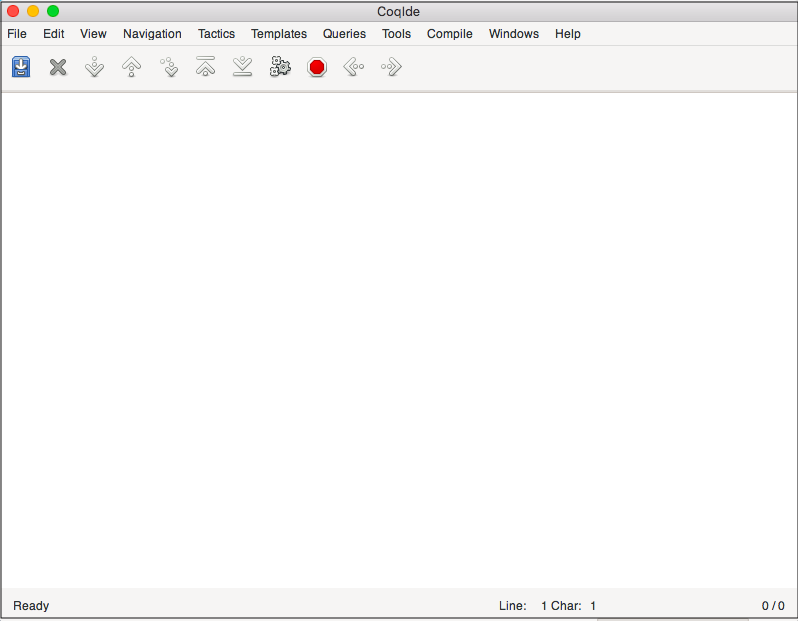
\includegraphics[width=\halfsize]
        		{CoqScreenshots/emptyIDE.png}
	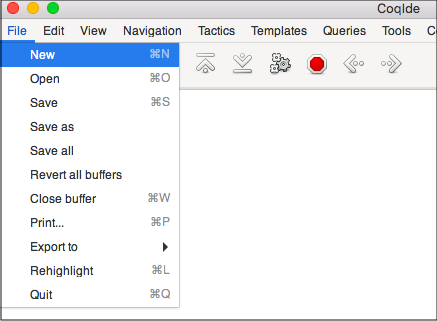
\includegraphics[width=\halfsize]
        		{CoqScreenshots/FixEmptyIDE.png}}
        
        \label{fig: IDEempty} 
        \captionof{figure}{CoqIDE v8.10.2  
        (a) empty IDE screen (b) getting new scratch script buffer open }
\end{minipage}

~\\~\\ 
Go to \TT{File} then \TT{New} to get a new scratch script buffer open if you've accidentally closed out all of your script buffers. Alternately, you can go to \TT{File} then \TT{Open} if you'd like to open a saved file. 





\subsection{Can't close \TT{Load File} window}

\begin{minipage}{\linewidth}
\center{
	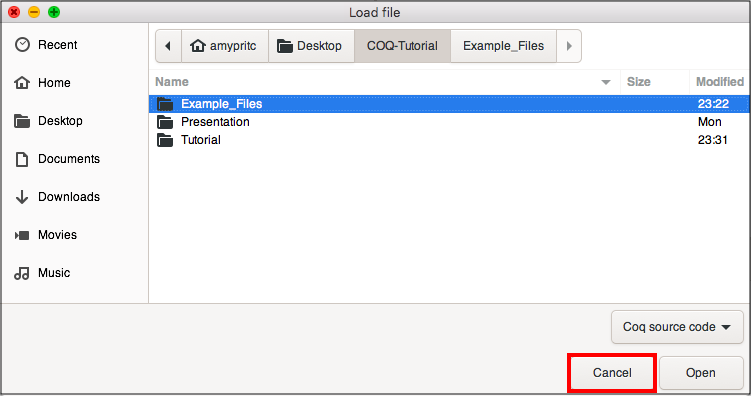
\includegraphics[width=\linewidth]
        		{CoqScreenshots/load_file.png}}
        \label{fig: LoadFile} 
        \captionof{figure}{CoqIDE v8.10.2 Load File window}
\end{minipage}

~\\~\\
If the \TT{Load File} window won't close using the red X in the upper left-hand corner, 
use the \TT{Cancel} button in the lower right (outlined in red). 






\subsection{File didn't save with the \TT{.v} extension}

When saving a new buffer, you need to ensure you add the \TT{.v} extension to the file name. 
If you forgot to do this, you can either use \TT{File} then \TT{Save as} (then reopen the correctly named program)
or modify the name outside of the CoqIDE (i.e. command line or file explorer such as Finder for MacOS). 






\subsection{Can't get pre-defined datatype to work}

Try using the full name of the type - i.e.
\\ \TT{nat}: use \TT{Datatype.nat}
\\ \TT{list}: use \TT{Datatype.list}






\subsection{Copy/paste program from a file into CoqIDE - program not working}

Copying from a file and pasting into the CoqIDE can cause some issues. 
The most common one I have found is that any use of the underscore (i.e., \TT{\_}) tends to get erased. 
If you are looking to try out code from this tutorial, the best way to do so is to use the provided example files, 
as these have all been tested to ensure they work properly in the CoqIDE.  




\subsection{CoqIDE running very slow}

I do not have a solution to this, but have seen the CoqIDE run very slowly on a VM running linux 
(to the point that it was nearly impossible to use). 
Installing on Windows and Mac with version 8.10.2 should work well with a pretty good response time 
(load libraries will take slightly longer than just stepping through code, but is still within reason). 
If you run into this issue, try reinstalling or heading over to the Coq website (\url{https://coq.inria.fr}) 
for assistance.  


\subsection{Can't get file to open in CoqIDE from file explorer}

The CoqIDE, from my experience, won't allow you to open a file in the IDE from a file explorer (i.e., Finder on MacOS). 
To open a file, do so directly from the CoqIDE by going to \TT{File} then \TT{Open}, then navigating to the appropriate 
location where the file is stored in the pop-up window, and proceeding to open it from there. 






